\documentclass{article}
\usepackage{tikz}
\usetikzlibrary{arrows.meta,positioning,calc,shapes.geometric}
\pagestyle{empty}
\begin{document}
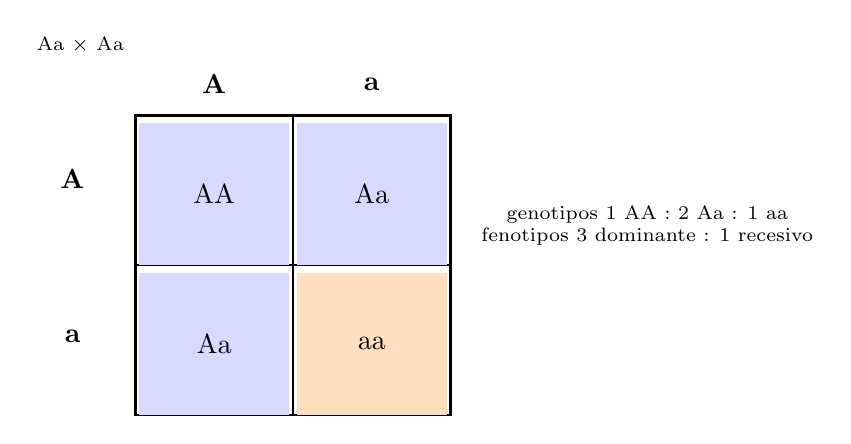
\begin{tikzpicture}
\tikzset{every node/.append style={align=center}}

\node[font=\scriptsize] at (0.5,3.9) {Aa $\times$ Aa};
\node[font=\bfseries] at (2.2,3.4) {A}; \node[font=\bfseries] at (4.2,3.4) {a};
\node[font=\bfseries] at (0.4,2.2) {A}; \node[font=\bfseries] at (0.4,0.2) {a};
\draw[thick] (1.2,3.0) rectangle (5.2,-0.8); \draw[thick] (3.2,3.0) -- (3.2,-0.8); \draw[thick] (1.2,1.1) -- (5.2,1.1);
\node[fill=blue!15, minimum width=1.9cm, minimum height=1.8cm] at (2.2,2.0) {AA}; \node[fill=blue!15, minimum width=1.9cm, minimum height=1.8cm] at (4.2,2.0) {Aa};
\node[fill=blue!15, minimum width=1.9cm, minimum height=1.8cm] at (2.2,0.1) {Aa}; \node[fill=orange!25, minimum width=1.9cm, minimum height=1.8cm] at (4.2,0.1) {aa};
\node[font=\scriptsize, align=center] at (7.7,1.6) {genotipos 1 AA : 2 Aa : 1 aa\\ fenotipos 3 dominante : 1 recesivo};

\end{tikzpicture}
\end{document}
